<<<<<<< HEAD
%!TEX TS-program = pdflatex
\documentclass[aspectratio=169]{beamer}
\usepackage[utf8]{inputenc}
\usepackage[T1]{fontenc}
\title{There Is No Largest Prime Number}
\date[ISPN ’80]{27th International Symposium of Prime Numbers}
\author[Euclid]{Euclid of Alexandria \texttt{euclid@alexandria.edu}}
%
\usetheme{uow}
=======
\documentclass[aspectratio=1610]{beamer}
\usepackage[scale=2.5]{ccicons}
\usepackage{tikz}
   \usetikzlibrary{matrix}

\usepackage{chemmacros}
\newcommand{\key}[1]{\texttt{\color{UOWorange}#1}} 
\newcommand{\val}[1]{\texttt{\color{UOWblue}#1}} 
\newcommand{\command}[1]{\texttt{\color{UOWdarkgreen}#1}} 

\title{The Presentation Title}
\subtitle{A nice little subtitle}
\author[Thomas]{Thomas M Griffiths}
\institute{School of Chemistry}
\date{}

\usetheme[]{uow}
%\usetheme{Madrid}
>>>>>>> dev

\begin{document}

\maketitle

\begin{frame}[fragile]
\frametitle{Typography}
\begin{verbatim}
The theme provides sensible defaults to 
\emph{emphasize} text, \alert{accent} parts 
or show \textbf{bold} results.
\end{verbatim}
\begin{center} \textit{becomes} \end{center}
The theme provides sensible defaults to \emph{emphasize} text, \alert{accent} parts or show \textbf{bold} results.
\end{frame}

\begin{frame}
   \frametitle{Columns, Lists and Images}
   \begin{columns}
      \begin{column}{0.5\textwidth}
         \begin{enumerate}
            \item Imidazopyrazinone backbone (in red).
            \item Most common substrate in \textbf{marine bioluminescence}.
            \item Proposed antioxidant capabilities.
            \item Unknown uptake or synthetic pathway in nature.
            \item $y=mx+b$ is some example mathematics.
         \end{enumerate}
      \end{column}
      \begin{column}{0.5\textwidth}
         \centering
         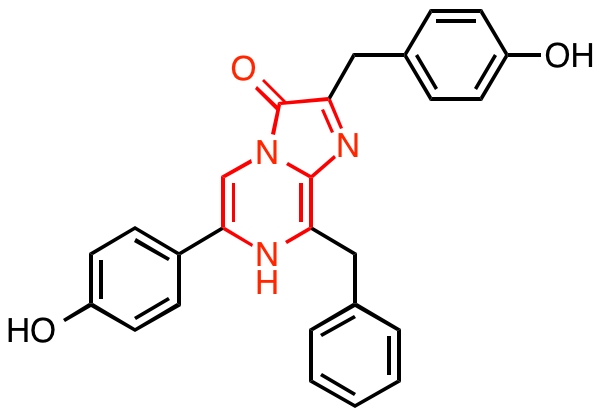
\includegraphics[width=0.8\textwidth]{coelenterazine.png}
      \end{column}
   \end{columns}
\end{frame}


%\begin{frame}{Itemised Lists With Columns}
%   \begin{columns}[T]
%      \begin{column}{0.48\textwidth}
%      Lorem ipsum dolor sit amet, consetetur sadipscing elitr, sed diam nonumy eirmod tempor invidunt ut labore et dolore magna aliquyam erat, sed diam voluptua. At vero eos et accusam et justo duo dolores et ea rebum. Stet clita kasd gubergren, no sea takimata sanctus est Lorem ipsum dolor sit amet. Lorem ipsum dolor sit amet, consetetur sadipscing elitr, sed diam nonumy eirmod tempor.
%      \end{column}
%      \begin{column}{0.48\textwidth}
%      \begin{itemize}
%         \item One point
%         \item Another point
%         \item And a \alert{third}!
%      \end{itemize}
%      \end{column}
%   \end{columns}
%\end{frame}
%
%
\begin{frame}
\frametitle{Blocks}
   \begin{block}{Blocks are Used for Emphasis in Beamer}
      Anything can go in a block.
      \begin{itemize}
         \item Bullet points.
         \item For demonstration,
         \item or to summarise something.
      \end{itemize}
   \end{block}
\end{frame}

<<<<<<< HEAD
\begin{frame} 
\frametitle{There Is No Largest Prime Number} 
\framesubtitle{The proof uses \textit{reductio ad absurdum}.} 
\begin{theorem}
There is no largest prime number. \end{theorem} 
\begin{enumerate} 
\item<1-| alert@1> Suppose $p$ were the largest prime number. 
\item<2-> Let $q$ be the product of the first $p$ numbers. 
\item<3-> Then $q+1$ is not divisible by any of them. 
\item<1-> But $q + 1$ is greater than $1$, thus divisible by some prime
number not in the first $p$ numbers.
\end{enumerate}
=======

\begin{frame}[fragile]
\frametitle{Blocks}
   \begin{columns}
      \begin{column}{0.48\textwidth}
         \begin{block}{Blocks}
            Anything can go in a block.
            \begin{itemize}
               \item Bullet points.
               \item For demonstration,
               \item or to summarise something.
            \end{itemize}
         \end{block}
      \end{column}
      \begin{column}{0.48\textwidth}
         \footnotesize
         \begin{verbatim}
\begin{block}{Blocks are Used for Emphasis in Beamer}
   Anything can go in a block.
   \begin{itemize}
      \item Bullet points.
      \item For demonstration,
      \item or to summarise something.
   \end{itemize}
\end{block}
         \end{verbatim}
      \end{column}
   \end{columns}
>>>>>>> dev
\end{frame}


\begin{frame}
\frametitle{More Blocks}
   \begin{alertblock}{This is an Alert Block}
      Alert blocks are usually used for some key point to be highlighted in a talk.
      A chemical reaction for example:\footnote{This example needs the \texttt{chemmacros} package, If you're writing about chemistry the author recommends it.}
      \begin{equation}
         \ch{CH4 + 2 O2 -> 2 H2O + CO2}
      \end{equation}
   \end{alertblock}
\end{frame}


\begin{frame}
\frametitle{Even More Blocks}
   \begin{exampleblock}{This is an Example Block}
      The example block is usually used for examples. Here I find the solutions to a quadratic equation.
      \begin{align*}
         2x^2 + 2x - 4 & = 0 \\
         a=2, \quad b & =2, \quad c=-4\\
         x & =\frac{-b\pm\sqrt{b^2-4ac}}{2a} \\
         x & =-2 \text{ or } 1
      \end{align*}
   \end{exampleblock}
\end{frame}


\begin{frame}\footnotesize
   The Beamer implementation 'UOWtheme' is copyright (CC BY-NC-SA 4.0 Int) 2015 by T. M. Griffiths under the \href{http://creativecommons.org/licenses/by-sa/4.0/}{Creative Commons Attribution-Share Alike 4.0 International License}\footnote{\url{http://creativecommons.org/licenses/by-nc-sa/4.0/}}.
   
   \begin{center}\ccbysa\end{center}
   
   The crest and associated branding of the University of Wollongong is copyright and the property of the University of Wollongong. As the core identifier of the university its use is governed by the university's brand and visual identity guidelines which can be found \href{http://www.uow.edu.au/about/brand/uowlogo/index.html}{online}\footnote{\url{http://www.uow.edu.au/about/brand/uowlogo/index.html}}.
   
\end{frame}
\end{document}
